\documentclass[12pt]{article}

	\usepackage{lmodern}
\usepackage{amssymb}
\usepackage{graphicx}
\usepackage{amsmath}
\usepackage{multirow}
\usepackage{mathtools}
\usepackage{placeins}
\usepackage{lscape}
\usepackage{geometry}
\usepackage{dcolumn}
\usepackage[utf8]{inputenc}
\usepackage{hyperref}
\usepackage{tabularx}
\usepackage{nicematrix}
\usepackage{calc}
\usepackage{qtree}
\usepackage{tikz}
\usepackage{setspace}
\usepackage[utf8]{inputenc}

	
	\usepackage{fullpage} %sets 1-in margins
	\newcommand{\tab}{\hspace*{2em}} %creates a \tab command, gives you horizontal space

	\setlength\parindent{0em} %sets indent
	 %\pagestyle{empty} %turns off page numbering on all pages

\makeatletter
\setlength{\@fptop}{0pt}
\setlength{\@fpbot}{0pt plus 1fil}
\makeatother

\title{SOFR and Crowding-Out Effect}
\date{}
\author{}

\begin{document}


\section{Response of SOFR and LIBOR to Gov't Borrowing}
\begin{center}
\footnotesize
\begin{tabular}{@{\extracolsep{5pt}}lD{.}{.}{-3} D{.}{.}{-3} D{.}{.}{-3} D{.}{.}{-3} } 
\\[-1.8ex]\hline 
\hline \\[-1.8ex] 
\multicolumn{5}{c}{\textit{Panel A: Gov't debt outstanding as the measure of borrowing}} \\ 
\cline{1-5} \\
 & \multicolumn{4}{c}{\textit{Dependent variable:}} \\ 
 \cline{2-5} \\
\\[-1.8ex] & \multicolumn{2}{c}{SOFR} & \multicolumn{2}{c}{LIBOR} \\ 
\\[-1.8ex] & \multicolumn{1}{c}{(1)} & \multicolumn{1}{c}{(2)} & \multicolumn{1}{c}{(3)} & \multicolumn{1}{c}{(4)}\\ 
\hline \\[-1.8ex] 
$\Delta$log debt & 386.758^{***} & 381.218^{***} & -34.675^{**} & -33.695^{**} \\ 
  & (65.325) & (65.971) & (15.578) & (15.654) \\ 
SOFR(-1)  &  & 0.031 &  &  \\ 
  &  & (0.025) &  &  \\ 
LIBOR(-1)  &  &  &  & -0.144^{***} \\ 
  &  &  &  & (0.026) \\ 
  Constant & -0.241^{***} & -0.236^{***} & 0.011 & 0.011 \\ 
  & (0.076) & (0.077) & (0.018) & (0.018) \\ 
 \hline \\[-1.8ex] 
Observations & \multicolumn{1}{c}{1,526} & \multicolumn{1}{c}{1,520} & \multicolumn{1}{c}{1,489} & \multicolumn{1}{c}{1,464} \\ 
R$^{2}$ & \multicolumn{1}{c}{0.022} & \multicolumn{1}{c}{0.023} & \multicolumn{1}{c}{0.003} & \multicolumn{1}{c}{0.024} \\ 
Adjusted R$^{2}$ & \multicolumn{1}{c}{0.022} & \multicolumn{1}{c}{0.021} & \multicolumn{1}{c}{0.003} & \multicolumn{1}{c}{0.023} \\ 
Residual Std. Error & \multicolumn{1}{c}{2.929 (df = 1524)} & \multicolumn{1}{c}{2.933 (df = 1517)} & \multicolumn{1}{c}{0.689 (df = 1487)} & \multicolumn{1}{c}{0.686 (df = 1461)} \\ 
[.8ex]\hline 
\hline \\[-1.8ex] 
\multicolumn{5}{c}{\textit{Panel B: Treasuries outstanding as the measure of borrowing}} \\ 
\cline{1-5} \\
 & \multicolumn{4}{c}{\textit{Dependent variable:}} \\ 
 \cline{2-5} \\
\\[-1.8ex] & \multicolumn{2}{c}{SOFR} & \multicolumn{2}{c}{LIBOR} \\ 
\\[-1.8ex] & \multicolumn{1}{c}{(1)} & \multicolumn{1}{c}{(2)} & \multicolumn{1}{c}{(3)} & \multicolumn{1}{c}{(4)}\\ 
\hline \\[-1.8ex] 
$\Delta$log treasuries & 995.000^{***} & 994.614^{***} & -72.438^{***} & -66.848^{***} \\ 
  & (90.566) & (88.833) & (19.771) & (19.647) \\ 
SOFR(-1) &  & 0.177^{***} &  &  \\ 
  &  & (0.028) &  &  \\ 
LIBOR(-1) &  &  &  & -0.154^{***} \\ 
  &  &  &  & (0.030) \\ 
  Constant & -0.358^{***} & -0.314^{***} & 0.014 & 0.013 \\ 
  & (0.085) & (0.084) & (0.019) & (0.019) \\ 
 \hline \\[-1.8ex] 
Observations & \multicolumn{1}{c}{1,134} & \multicolumn{1}{c}{1,129} & \multicolumn{1}{c}{1,100} & \multicolumn{1}{c}{1,079} \\ 
R$^{2}$ & \multicolumn{1}{c}{0.096} & \multicolumn{1}{c}{0.129} & \multicolumn{1}{c}{0.012} & \multicolumn{1}{c}{0.036} \\ 
Adjusted R$^{2}$ & \multicolumn{1}{c}{0.096} & \multicolumn{1}{c}{0.127} & \multicolumn{1}{c}{0.011} & \multicolumn{1}{c}{0.034} \\ 
Residual Std. Error & \multicolumn{1}{c}{2.826 (df = 1132)} & \multicolumn{1}{c}{2.770 (df = 1126)} & \multicolumn{1}{c}{0.613 (df = 1098)} & \multicolumn{1}{c}{0.608 (df = 1076)} \\ 
\hline 
\hline \\[-1.8ex] 
\textit{Note:}  & \multicolumn{4}{r}{$^{*}$p$<$0.1; $^{**}$p$<$0.05; $^{***}$p$<$0.01} \\ 
\end{tabular} 
\end{center}


\newpage
\section{The Scarcity Value of Treasury Collateral}
\subsection{Segments of Markets Underlying SOFR}
The transactions underlying SOFR comprises two segments: bilateral repo and tri-party repo. In a bilateral repo, the settlement is handled directly by the trading parties rather than by a third-party clearing bank as in a triparty repo. Tri-party transactions are secured by General Collateral (GC) pools of accepted Treasury securities, any of which can be delivered as collateral by the cash borrower.  Unlike tri-pary transaction,  bilateral transactions feature Specific Collateral (SC) as lenders and borrowers can designate specific securities as collateral.  Therefore,  the incentive for lenders entering the bilateral repo market can be to seek a specific security.  A so-called collateral scarcity premium arises in bilateral transactions. \footnote{Infante and Saravay (2020) and D’Amico et al.  (2018) provide empirical evidence for treasury collateral scarcity.} \\
\begin{center}
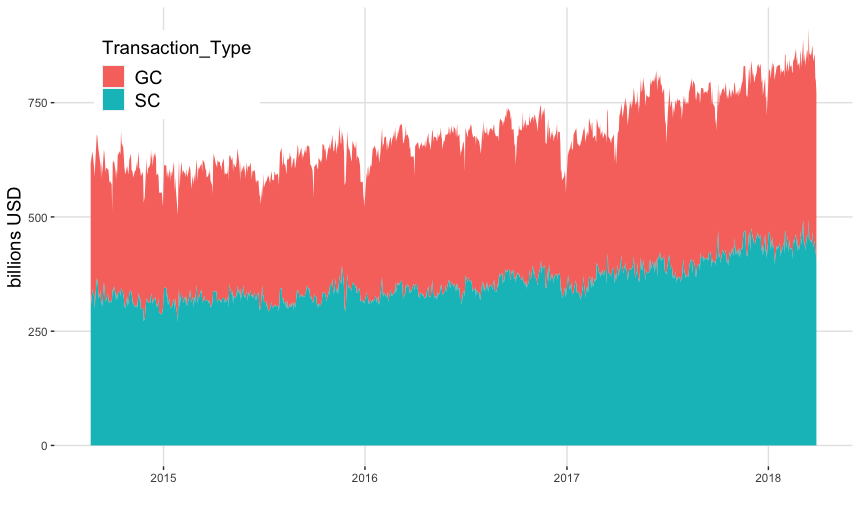
\includegraphics[scale=.5]{fig1.png}
\end{center}


\subsection{Treasuries Outstanding and Scarcity Value}
Intuitively,  when the volume of outstanding Treasuries is larger,  the Treasuries as collateral become less scarcity,  so the rate spread between bilateral repo transactions and tri-party repo transactions increases.  

\begin{center}
\begin{tabular}{@{\extracolsep{5pt}}lD{.}{.}{-3} D{.}{.}{-3} } 
\\[-1.8ex]\hline 
\hline \\[-1.8ex] 
 & \multicolumn{2}{c}{\textit{Dependent variable:}} \\ 
\cline{2-3} 
\\[-1.8ex] & \multicolumn{2}{c}{SC repo rate - GC repo rate} \\ 
\\[-1.8ex] & \multicolumn{1}{c}{(1)} & \multicolumn{1}{c}{(2)}\\ 
\hline \\[-1.8ex] 
$\Delta$log treasuries & 1,280.301^{***} & 1,321.397^{***} \\ 
  & (232.948) & (221.020) \\ 
$\Delta$log GC volume &  & -46.675^{***} \\ 
  &  & (4.473) \\ 
$\Delta$log SC volume&  & 6.483 \\ 
  &  & (4.377) \\ 
  Constant & -0.236 & -0.238 \\ 
  & (0.225) & (0.212) \\ 
 \hline \\[-1.8ex] 
Observations & \multicolumn{1}{c}{899} & \multicolumn{1}{c}{899} \\ 
R$^{2}$ & \multicolumn{1}{c}{0.033} & \multicolumn{1}{c}{0.138} \\ 
Adjusted R$^{2}$ & \multicolumn{1}{c}{0.031} & \multicolumn{1}{c}{0.135} \\ 
Residual Std. Error & \multicolumn{1}{c}{6.591 (df = 897)} & \multicolumn{1}{c}{6.230 (df = 895)} \\ 
\hline 
\hline \\[-1.8ex] 
\textit{Note:}  & \multicolumn{2}{r}{$^{*}$p$<$0.1; $^{**}$p$<$0.05; $^{***}$p$<$0.01} \\ 
\end{tabular} 
\end{center}




\end{document}